\chapter{Circular Motion, continued}
\section{Review of Circular Motion Basics}
define rigid body
recall angular kinematics formulas, recall arc length
\section{Torque}
Let's think about pushing a box along a frictionless surface. There is a linear relationship between how hard you push and how much the box accelerates. What if, instead, you apply the same force to a merry-go-round fixed at a central pivot? Where can you push the merry-go-round for the most rotation. Obviously you cannot push the merry-go-round linearly, so how far will the merry-go-round rotate? All of these questions can be answered by the concept of \emph{torque}. 
\begin{figure}[H]
\centering
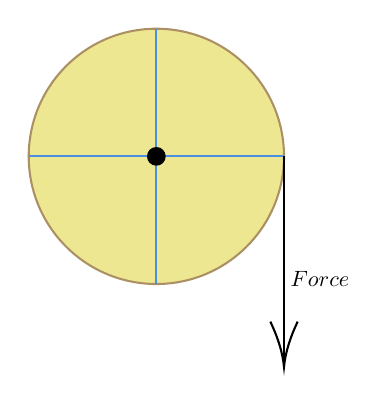
\begin{tikzpicture}[x=0.75pt,y=0.75pt,yscale=-1,xscale=1]

%Shape: Circle
\draw[color={rgb,255:red,170;green,144;blue,99},draw opacity=1,
      fill={rgb,255:red,238;green,231;blue,145},fill opacity=1]
(14,76.5) .. controls (14,42.53) and (41.53,15) .. (75.5,15)
.. controls (109.47,15) and (137,42.53) .. (137,76.5)
.. controls (137,110.47) and (109.47,138) .. (75.5,138)
.. controls (41.53,138) and (14,110.47) .. (14,76.5) -- cycle ;

%Axes/diameter lines (blue)
\draw[color={rgb,255:red,74;green,144;blue,226},draw opacity=1]
(75.5,138) -- (75.5,15) ;
\draw[color={rgb,255:red,74;green,144;blue,226},draw opacity=1]
(14,76.5) -- (137,76.5) ;

%Center point
\draw[fill={rgb,255:red,0;green,0;blue,0},fill opacity=1]
(71.5,76.5) .. controls (71.5,74.29) and (73.29,72.5) .. (75.5,72.5)
.. controls (77.71,72.5) and (79.5,74.29) .. (79.5,76.5)
.. controls (79.5,78.71) and (77.71,80.5) .. (75.5,80.5)
.. controls (73.29,80.5) and (71.5,78.71) .. (71.5,76.5) -- cycle ;


%Force arrow
\draw (137,76.5) -- (137,176) ;
\draw[shift={(137,178)}, rotate=270, color={rgb,255:red,0;green,0;blue,0}, line width=0.75]
(21.86,-6.58) .. controls (13.9,-2.79) and (6.61,-0.6) .. (0,0)
.. controls (6.61,0.6) and (13.9,2.79) .. (21.86,6.58);

%Label
\draw (139,130.65) node [anchor=north west,inner sep=0.75pt,xscale=0.8,yscale=0.8] {$Force$};

\end{tikzpicture}
\caption{Merry-go-round with a singular applied force.}
\end{figure}

\index{torque}
Torque is the concept of \emph{rotational force}. Applying a torque to a surface, a \emph{rigid body}, that has a fixed rotational pivot will cause the rigid body to \emph{accelerate} around the pivot, ultimately producing an \emph{angular acceleration}. 

Imagine pushing open a door that is bound to a hinge on one side of the door. Pushing open the door at a point close to the hinge will require large amount of Torque, while pushing closer to the door handle and farther away from the hinge is much easier to do, and requires less Torque. 

Alternatively, think of a wrench rotating a large bolt. It will require more force from your arm closer towards the pivot, while pushing at the edge of the wrench will require less force to produce an equivalent torque.

FIXME Door diagram or wrench diagram or both

\index{torques}\index{torque}
\begin{mdframed}[frametitle = {Torque}, style = important]
Torque, represented through the greek letter \tau (tau), is defined as
\begin{equation}
    \tau = rF
    \label{eq:torque_perp}
\end{equation}
where $F$ is a force perpendicular to 
\begin{equation}
    \tau = r F \sin\theta
    \label{eq:torque_sin}
\end{equation}
Notice that the torque around a pivot depends on the distance from the pivot, $r$, and the angle from the radius vector \theta. The $\sin\theta$ indicates that only the \emph{perpendicular} part of the force impacts the torque. This is equivalent to the cross product of the two vectors:
\begin{equation}
    \tau = r \times F
    \label{eq:torque_cross}
\end{equation}
Torque has units of $\text{Newton-meters}$, but in this case, it is not an energy form, so cannot be equated to $\text{Joules}$. Torque is an \emph{vector}, not a scalar.
\end{mdframed}

Let's do an example proving this.

\textbf{Question}: A rod with a fixed end is being pulled by a tension force of $50 \,\text{N}$ at a $40^\circ$ angle from the horizontal, at a distance of $2 \,\text{m}$. Find the Torque on the rod.

% Diagram made with Mathcha
\tikzset{every picture/.style={line width=0.75pt}} % default line width


\begin{figure}[H]
\centering
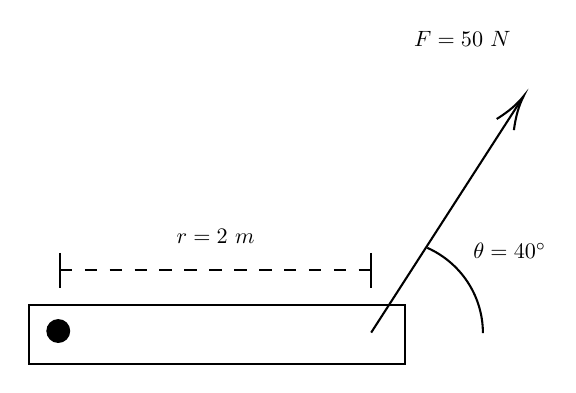
\begin{tikzpicture}[x=0.75pt,y=0.75pt,yscale=-1.5,xscale=1.5]
% Main diagram pieces (from the original)
%Shape: Rectangle
\draw (1,93) -- (122,93) -- (122,112) -- (1,112) -- cycle ;
%Shape: Circle
\draw[fill={rgb,255:red,0;green,0;blue,0},fill opacity=1]
  (7,101.5) .. controls (7,99.57) and (8.57,98) .. (10.5,98)
  .. controls (12.43,98) and (14,99.57) .. (14,101.5)
  .. controls (14,103.43) and (12.43,105) .. (10.5,105)
  .. controls (8.57,105) and (7,103.43) .. (7,101.5) -- cycle ;

%Shape: Arc (angle marker)
\draw[draw opacity=0]
  (129.02,74.78) .. controls (139.52,79.43) and (146.86,89.92) .. (146.89,102.15)
  -- (116.89,102.23) -- cycle ;
\draw
  (129.02,74.78) .. controls (139.52,79.43) and (146.86,89.92) .. (146.89,102.15) ;

%Force arrow
\draw (111,102) -- (158.92,27.68) ;
\draw[shift={(160,26)}, rotate=122.81, line width=0.75]
  (10.93,-3.29) .. controls (6.95,-1.4) and (3.31,-0.3) .. (0,0)
  .. controls (3.31,0.3) and (6.95,1.4) .. (10.93,3.29);

%Dashed radius/lever arm line
\draw[dash pattern={on 4.5pt off 4.5pt}] (11,82) -- (111,82) ;
\draw[shift={(111,82)}, rotate=180, line width=0.75] (0,5.59) -- (0,-5.59);
\draw[shift={(11,82)}, rotate=180,  line width=0.75] (0,5.59) -- (0,-5.59);

% Text nodes
\draw (143,72.4) node [anchor=north west,inner sep=0.75pt,xscale=0.8,yscale=0.8] {$\theta =40^{\circ }$};
\draw (124,4.4)  node [anchor=north west,inner sep=0.75pt,xscale=0.8,yscale=0.8] {$F=50\ \text{N}$};
\draw (61,71)    node [xscale=0.8,yscale=0.8] {$r=2\ \text{m}$};
\end{tikzpicture}
\caption{Main diagram.}
\end{figure}


\textbf{Answer}: Before just plugging in values, let's seperate the force vector into components. The component that pulls perpendicular to the axis is $50 \sin40^\circ$, while $50 \cos40^\circ$ of the force is applied \textit{pulling} the rod against the pivot, which produces no torque. 
% Diagram made with mathcha
\begin{figure}[H]
\centering

\begin{subfigure}{0.48\linewidth}
\centering
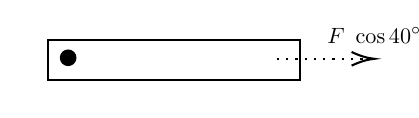
\begin{tikzpicture}[x=0.75pt,y=0.75pt,yscale=-1,xscale=1]
% Tight bounding box around this component
\path[use as bounding box] (200,85) rectangle (375,115);

%Shape: Rectangle
\draw (210,91) -- (331,91) -- (331,110) -- (210,110) -- cycle ;
%Shape: Circle
\draw[fill={rgb,255:red,0;green,0;blue,0},fill opacity=1]
  (216,99.5) .. controls (216,97.57) and (217.57,96) .. (219.5,96)
  .. controls (221.43,96) and (223,97.57) .. (223,99.5)
  .. controls (223,101.43) and (221.43,103) .. (219.5,103)
  .. controls (217.57,103) and (216,101.43) .. (216,99.5) -- cycle ;

%Straight line (cos component)
\draw[dash pattern={on 0.84pt off 2.51pt}] (320,100) -- (365,100) ;
\draw[shift={(367,100)}, rotate=180, color={rgb,255:red,0;green,0;blue,0}, line width=0.75]
  (10.93,-3.29) .. controls (6.95,-1.4) and (3.31,-0.3) .. (0,0)
  .. controls (3.31,0.3) and (6.95,1.4) .. (10.93,3.29);

% Label
\draw (367,93.6) node [anchor=south,inner sep=0.75pt,xscale=0.8,yscale=0.8] {$F\ \cos 40^{\circ }$};
\end{tikzpicture}
\caption{$F\cos\theta$}
\end{subfigure}
\hfill
%------------------------
% (b) Sine component
%------------------------
\begin{subfigure}{0.48\linewidth}
\centering
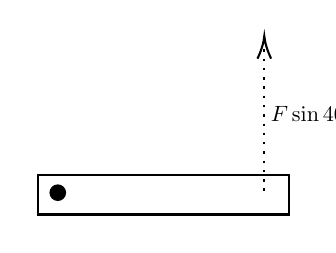
\begin{tikzpicture}[x=0.75pt,y=0.75pt,yscale=-1,xscale=1]
% Tight bounding box around this component
\path[use as bounding box] (405,20) rectangle (540,115);

%Shape: Rectangle
\draw (410,91) -- (531,91) -- (531,110) -- (410,110) -- cycle ;
%Shape: Circle
\draw[fill={rgb,255:red,0;green,0;blue,0},fill opacity=1]
  (416,99.5) .. controls (416,97.57) and (417.57,96) .. (419.5,96)
  .. controls (421.43,96) and (423,97.57) .. (423,99.5)
  .. controls (423,101.43) and (421.43,103) .. (419.5,103)
  .. controls (417.57,103) and (416,101.43) .. (416,99.5) -- cycle ;

%Straight line (sin component)
\draw[dash pattern={on 0.84pt off 2.51pt}] (519,26) -- (519,99) ;
\draw[shift={(519,24)}, rotate=90, color={rgb,255:red,0;green,0;blue,0}, line width=0.75]
  (10.93,-3.29) .. controls (6.95,-1.4) and (3.31,-0.3) .. (0,0)
  .. controls (3.31,0.3) and (6.95,1.4) .. (10.93,3.29);

% Label
\draw (521,61.5) node [anchor=west,inner sep=0.75pt,xscale=0.8,yscale=0.8] {$F\sin 40^{\circ }$};
\end{tikzpicture}
\caption{$F\sin\theta$}
\end{subfigure}

\caption{Components of the applied force.}
\end{figure}

Think back to the wrench example: you don't push or pull a wrench to loosen a bolt; you must apply a force \emph{tangential} or \emph{perpendicular} to the bolt to rotate it. 

Since only the perpendicular component contributes to the torque, we calculate the torque to be $\tau = 50 \sin40^\circ \,\text{N} \,(2 \text{m}) \approx 64.278 \,\text{Newton-meters}$


FIXME simple tangential torque
\subsection{Torque directions}
\index{torques!applied in opposite directions}
What happens when two torques are applied in \emph{opposite}? Let's take a look at the merry-go-round again, but this time applied with two torques.
% Mathcha
\begin{figure}[H]
\centering
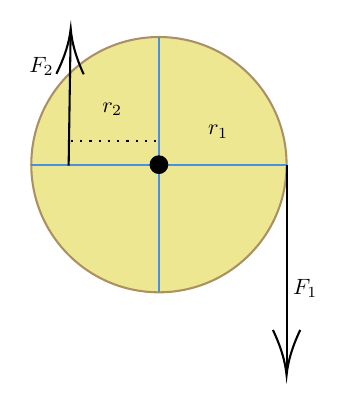
\begin{tikzpicture}[x=0.75pt,y=0.75pt,yscale=-1,xscale=1]

%Shape: Circle
\draw[color={rgb,255:red,170;green,144;blue,99},draw opacity=1,
      fill={rgb,255:red,238;green,231;blue,145},fill opacity=1]
(214,91.5) .. controls (214,57.53) and (241.53,30) .. (275.5,30)
.. controls (309.47,30) and (337,57.53) .. (337,91.5)
.. controls (337,125.47) and (309.47,153) .. (275.5,153)
.. controls (241.53,153) and (214,125.47) .. (214,91.5) -- cycle ;

%Axes/diameter lines (blue)
\draw[color={rgb,255:red,74;green,144;blue,226},draw opacity=1]
(275.5,153) -- (275.5,30) ;
\draw[color={rgb,255:red,74;green,144;blue,226},draw opacity=1]
(214,91.5) -- (337,91.5) ;
%Center point
\draw[fill={rgb,255:red,0;green,0;blue,0},fill opacity=1]
(271.5,91.5) .. controls (271.5,89.29) and (273.29,87.5) .. (275.5,87.5)
.. controls (277.71,87.5) and (279.5,89.29) .. (279.5,91.5)
.. controls (279.5,93.71) and (277.71,95.5) .. (275.5,95.5)
.. controls (273.29,95.5) and (271.5,93.71) .. (271.5,91.5) -- cycle ;


%Force F1 (downward)
\draw (337,91.5) -- (337,191) ;
\draw[shift={(337,193)}, rotate=270, color={rgb,255:red,0;green,0;blue,0}, line width=0.75]
(21.86,-6.58) .. controls (13.9,-2.79) and (6.61,-0.6) .. (0,0)
.. controls (6.61,0.6) and (13.9,2.79) .. (21.86,6.58);

%Force F2 (upward, offset)
\draw (232,92) -- (232.97,28) ;
\draw[shift={(233,26)}, rotate=90.87, color={rgb,255:red,0;green,0;blue,0}, line width=0.75]
(21.86,-6.58) .. controls (13.9,-2.79) and (6.61,-0.6) .. (0,0)
.. controls (6.61,0.6) and (13.9,2.79) .. (21.86,6.58);

%Dashed radius segment and labels
\draw[dash pattern={on 0.84pt off 2.51pt}] (233,80) -- (277,80) ;
\draw (298,71.4) node [anchor=north west,inner sep=0.75pt,xscale=0.8,yscale=0.8] {$r_{1}$};
\draw (247,60.4) node [anchor=north west,inner sep=0.75pt,xscale=0.8,yscale=0.8] {$r_{2}$};

%Force labels
\draw (339,145.65) node [anchor=north west,inner sep=0.75pt,xscale=0.8,yscale=0.8] {$F_{1}$};
\draw (225.91,44.2) node [anchor=east,inner sep=0.75pt,xscale=0.8,yscale=0.8] {$F_{2}$};

\end{tikzpicture}
\caption{Merry-go-round with 2 forces in opposing directions.}
\end{figure}

Torques applied in opposition act \emph{in opposite directions along the axis of rotation}. As torque is a vector defined by the \emph{cross product equation}~\ref{eq:torque_cross}, so its direction is perpendicular to the plane formed by position vector and force which the plane live on. In problems, you will typically see the terms \emph{out of} ($\odot$), or \emph{into} ($\otimes$), the page, corresponding to the $+z$ or $-z$ directions, respectively. Remember these terms by the following visualiations: the out of symbol (\odot) looks like the tip of a feathered dart coming at you, while the into symbol (\otimes) looks like the feathers of a dart. 

To determine which direction a given torque points, one first identifies the sense of rotation the force would produce if acting alone: a force that tends to rotate the object counterclockwise in the plane produces a torque vector pointing out of the page, while a force that tends to rotate the object clockwise produces a torque vector pointing into the page. When two torques are opposite, one must therefore cause clockwise rotation and the other counterclockwise rotation, leading to torque vectors that are equal in line of action but opposite in direction. 

The \emph{net torque}\index{net torque} is the sum of all torques present, similar to how net force is the sum of all forces. Counterclockwise torques are positive, while clockwise torques are negative. Using our merry go round example, we have $F_2$ is \odot while $F_1$ is \otimes.
\begin{align*}
    \tau_{\text{net}} &= \sum \tau \\
    &=+(F_2)(r_2) - (F_1)(r_1)
\end{align*}
Because we know $\tau_1 > \tau_2$, the net torque is going to be negative, or \otimes and clockwise.


FIXME exercise 
\section{Moment of Inertia and }
We know Newton's Second Law by heart now, $F_{net} = ma$. You probably could recite it in your sleep, but what about a rotational equivalent. Recall that from our first circular motion chapter, we have the equation $a = r \alpha$. Let's do some conversions to get this into an angular form:
\begin{align}
    F &= ma \notag \\
    F &= mr\alpha \notag \\
    rF &= mr^2\alpha \notag \\
    \tau &= mr^2\alpha \label{eq:rotNewt2ndLaw}
\end{align}

From Equation~\ref{eq:rotNewt2ndLaw}, we can derive that the ``mass equivalent'' is $mr^2$, since $m$ is multiplied by $a$ in the linear $F=ma$, while $mr^2$ is muliplied by $\alpha$. Thus, we can state that for a point of distance $r$ from the pivot (or axis of rotation), that singular point has \emph{rotation inertia}, also called \emph{moment of inertia}, is defined as $mr^2$. For all point masses on an object, the total inertia is the sum of all point masses of the object.
\begin{mdframed}[frametitle = {Moment of Inertia}, style = important]
    A mass's total moment of inertia is given by the sum of each mass multiplied the distance from the axis of rotation squared.
    \begin{equation}
        I = \sum m r^2\label{eq:momentInertiaSum}
    \end{equation}
    for continuous, solid objects, this becomes
    \begin{equation}
        I = \int r^2 \, dm \label{eq:momentInertiaIntegral}
    \end{equation}
\end{mdframed}
From Equations~\ref{eq:momentInertiaSum} and \ref{eq:momentInertiaIntegral}, we see that mass farther from the axis matters much more than anything closer to the pivot. Or, for two objects, one solid (mass spread evenly throughout) and the other a hollow cylinder or hoop (mass confined to the edges), the hollow cylinder will have a greater moment of inertia.

By finding the net rotational inertia of an object, we can create an equation for the rotational equivalent of Newton's Second Law:
\begin{equation}
    \sum \tau = \tau_{net} = I \alpha
\end{equation}
FIXME Here is a chart of various moments of Inertia and their respective axes of rotation
FIXME hollow versus solid objects rolling
FIXME torque and moment of inertua and ang accel eqation 

\section{Parallel-Axis Theorem}
